\documentclass[10pt,pdf,hyperref={unicode}]{beamer}

\usepackage[normalem]{ulem}
\usepackage{qrcode}
\usepackage{array}
\usepackage[T2A]{fontenc}
\usepackage[utf8]{inputenc}
\usepackage{colortbl}
\usepackage{minted}
\usepackage{listings}
\usepackage{tcolorbox}

\setbeamertemplate{navigation symbols}{}

\usetheme{default}

\usepackage{array}
\newcolumntype{L}[1]{>{\raggedright\let\newline\\\arraybackslash\hspace{0pt}}m{#1}}
\newcolumntype{C}[1]{>{\centering\let\newline\\\arraybackslash\hspace{0pt}}m{#1}}
\newcolumntype{R}[1]{>{\raggedleft\let\newline\\\arraybackslash\hspace{0pt}}m{#1}}

\definecolor{shadecolor}{RGB}{210,210,210}
\newcommand{\asm}[1]{\mintinline{gas}{#1}}

\newcommand{\qrlinkframe}[2]{\begin{frame}{#1}
\center\qrcode[hyperlink,height=75px]{#2}
\end{frame}}

\title{Семинар 19: Linux networking}
\date{30 апреля, 2020}


\begin{document}

\begin{frame}
  \titlepage
\end{frame}

\begin{frame}{Протоколы}
\begin{itemize}
    \item Современные сети строятся на основе \emph{протоколов}
    \item Каждый протокол -- абстракция над другим протоколом (более низким) для решения какой-то проблемы
    \item Поэтому иногда говорят \emph{стек протоколов}
\end{itemize}
\end{frame}


\begin{frame}{Модель OSI}
\begin{itemize}
    \item Разделяет современные протоколы на 7 уровней
    \item Physical layer, L1
    \item Data link layer, L2
    \item Network layer, L3
    \item Transport layer, L4
    \item Тут немного пропустим :D
    \item Application layer, L7
\end{itemize}
\end{frame}


\begin{frame}{Модель OSI: physical layer}
\begin{itemize}
    \item Самый нижний слой
    \item Описывает то, как данные будут переданы через физическую среду
    \item Протоколы:
    \item Bluetooth
    \item Ethernet physical layer: Ethernet over twisted pair, Fast Ethernet, Gigabit Ethernet, ...
    \item IEEE 802.11
\end{itemize}
\end{frame}

\begin{frame}{Модель OSI: link layer}
\begin{itemize}
    \item Строится поверх L1
    \item Обеспечивает обмен данными между узлами в одной сети LAN (local area network) или WAN (wide area network)
    \item На этом уровне появляется \emph{канальный адрес (link address)}, например, MAC-адрес
    \item IEEE 802.11
    \item Ethernet
    \item На этом уровне работают, например, сетевые коммутаторы (свитчи)
\end{itemize}
\end{frame}


\begin{frame}{Модель OSI: network layer}
\begin{itemize}
    \item Обеспечивает связь между разными LAN и WAN
    \item На этом уровне появляется \emph{сетевой адрес (network address)}, например, IP-адрес
    \item Появляется понятие \emph{маршрутизации}
    \item Основной протокол -- Internet Protocol (IP)
\end{itemize}
\end{frame}

\begin{frame}{IP: IP-адрес и маски подсетей}
\begin{itemize}
    \item IPv4 адрес состоит из 32 бит (для IPv6 -- 128)
    \item Маска подсети -- множество IP-адресов с одинаковым префиксом
    \item CIDR-нотация: 10.0.0.0/8 -- общий префикс 8 бит
    \item Ещё иногда записывают так: 255.0.0.0
    \item Некоторые зарезервированные сети: 10.0.0.0/8, 127.0.0.1/8, 192.168.0.0./16
\end{itemize}
\end{frame}

\begin{frame}{IP: маршрутизация}
\begin{itemize}
    \item Теперь не все узлы сети связаны напрямую. Как передавать данные между ними?
    \onslide<2->\item Через другие узлы!
    \onslide<2->\item Передача между соседними узлами в IP-сети называется \emph{прыжком} или \emph{хопом (hop)}
    \onslide<2->\item Каждый узел сети имеет \emph{таблицу маршрутизации} (иногда даже несколько)
    \onslide<2->\item Эта таблица содержит маски подсетей и узел, куда нужно переслать данные
    \item AS -- это система IP-сетей и маршрутизаторов, управляемых одним или несколькими операторами, имеющими единую политику маршрутизации с Интернетом (\copyright Wikipedia)
\end{itemize}
\end{frame}

\begin{frame}{IP: маршрутизация}
\begin{itemize}
    \item AS -- это система IP-сетей и маршрутизаторов, управляемых одним или несколькими операторами, имеющими единую политику маршрутизации с Интернетом (\copyright Wikipedia)
    \item Точка обмена трафиком -- точки обмена трафиком между разными AS :)
    \item Одна из самых крупных в Европе и России -- MSK-IX
\end{itemize}
\end{frame}

\begin{frame}{IPv4: устройство пакета}
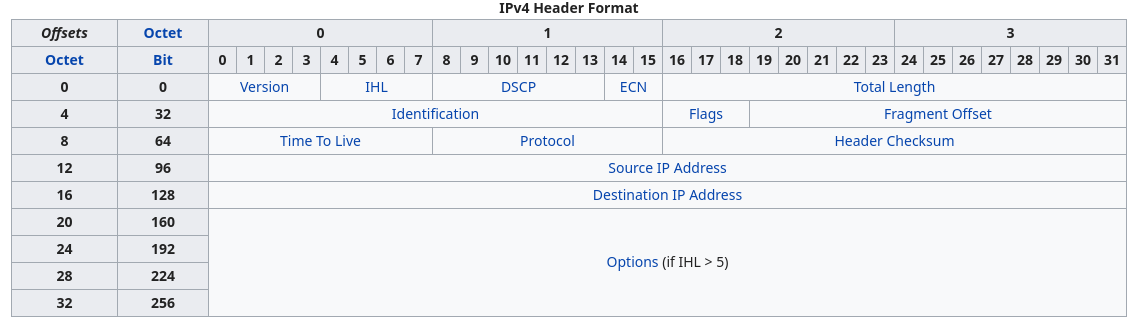
\includegraphics[width=300px]{ipv4_header.png}
\center{\small\copyright Wikipedia}
\end{frame}

\begin{frame}{IP: мини-бонус про TTL}
\begin{itemize}
    \item TTL -- tive-to-live
    \item Байт, который описывает максимальное количество прыжков в сети
    \item Если очередной хост уменьшил TTL до нуля, то пакет просто дропается, а отправителю посылается специальное сообщение по протоколу ICMP (TTL exceeded)
\end{itemize}
\end{frame}

\begin{frame}{IP: проблемы}
\begin{itemize}
    \item Не гарантирует доставку данных (packet loss)
    \item Не гарантирует порядок доставки (packet reordering)
    \item Не гарантирует, что пакет будет отправлен лишь один раз (packet duplication)
    \item Непонятно как реализовывать multitenancy IP протокола -- нельзя всем приложениям рассылать все IP-пакеты
\end{itemize}
\end{frame}


\begin{frame}{Модель OSI: transport layer}
\begin{itemize}
    \item Используется для передачи данных между различными приложениями на узлах сети
    \item Примеры: TCP, UDP, SCTP
\end{itemize}
\end{frame}


\begin{frame}{TCP}
\begin{itemize}
    \item Вводит понятие \emph{порта} приложения -- адрес получателя на IP-узле
    \item Обеспечивает надёжную доставку данных (reliable delivery)
    \item Обеспечивает порядок доставки и дедупликацию данных
    \item Connection-oriented -- приложения должны установить полнодуплексное \emph{соединение}
    \item Data stream -- данные передаются не отдельными пакетами, а непрерывным потоком
    \item Также обеспечивает congestion control и flow control
\end{itemize}
\end{frame}

\begin{frame}{TCP: устройство пакета}
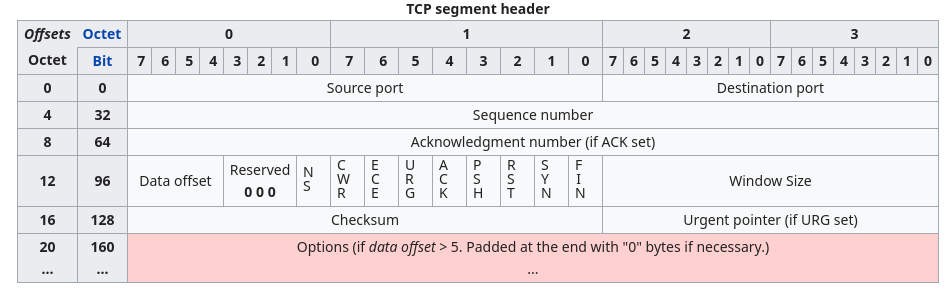
\includegraphics[width=300px]{tcp_header.png}
\end{frame}

\begin{frame}{TCP: 3-way handshake}
\begin{itemize}
    \item Механизм установки соединения -- <<рукопожатие>>
    \item Выполняется в три этапа:
\end{itemize}

\begin{enumerate}
    \onslide<2->\item Инициатор соединения (клиент) посылает пакет с флагом \textbf{SYN} серверу
    \onslide<3->\item Сервер посылает пакет с флагами \textbf{SYN} и \textbf{ACK} клиенту, а также \emph{sequence number}, с которого будут нумероваться все остальные байты
    \onslide<4->\item Клиент посылает \textbf{ACK}
\end{enumerate}
\end{frame}

\begin{frame}{UDP}
\begin{itemize}
    \item Не даёт никаких гарантий
    \item Пересылка осуществляется через пакеты (UDP datagrams)
    \item Используется там, где важна latency (например, онлайн игры)
    \item Или bandwidth (например, BitTorrent)
\end{itemize}
\end{frame}

\begin{frame}{Модель OSI: application layer}
\begin{itemize}
    \item Протоколы приложений (веб-браузеры, почтовые клиенты, игры)
    \item Один из самых известных -- HyperText Transfer Protocol (HTTP)
    \item Почтовые протоколы -- SMTP, POP3
    \item Secure Shell (SSH)
\end{itemize}
\end{frame}

\begin{frame}
\center\Huge{Теперь о том, как с этим работать в Linux}
\end{frame}

\begin{frame}
\center\Huge{Спасибо!}
\end{frame}


\end{document}
